% mnras_template.tex
%
% LaTeX template for creating an MNRAS paper
%
% v3.0 released 14 May 2015
% (version numbers match those of mnras.cls)
%
% Copyright (C) Royal Astronomical Society 2015
% Authors:
% Keith T. Smith (Royal Astronomical Society)

% Change log
%
% v3.0 May 2015
%    Renamed to match the new package name
%    Version number matches mnras.cls
%    A few minor tweaks to wording
% v1.0 September 2013
%    Beta testing only - never publicly released
%    First version: a simple (ish) template for creating an MNRAS paper

%%%%%%%%%%%%%%%%%%%%%%%%%%%%%%%%%%%%%%%%%%%%%%%%%%
% Basic setup. Most papers should leave these options alone.
\documentclass[a4paper,fleqn,usenatbib]{mnras}

% MNRAS is set in Times font. If you don't have this installed (most LaTeX
% installations will be fine) or prefer the old Computer Modern fonts, comment
% out the following line
\usepackage{newtxtext}
% Depending on your LaTeX fonts installation, you might get better results with one of these:
%\usepackage{mathptmx}
%\usepackage{txfonts}

% Use vector fonts, so it zooms properly in on-screen viewing software
% Don't change these lines unless you know what you are doing
\usepackage[T1]{fontenc}
\usepackage{ae,aecompl}


%%%%% AUTHORS - PLACE YOUR OWN PACKAGES HERE %%%%%

% Only include extra packages if you really need them. Common packages are:
\usepackage{graphicx}	% Including figure files
\usepackage{amsmath}	% Advanced maths commands
\usepackage{amssymb}	% Extra maths symbols
\usepackage{hyperref}
\usepackage{url}

%%%%%%%%%%%%%%%%%%%%%%%%%%%%%%%%%%%%%%%%%%%%%%%%%%

%%%%% AUTHORS - PLACE YOUR OWN COMMANDS HERE %%%%%

% Please keep new commands to a minimum, and use \newcommand not \def to avoid
% overwriting existing commands. Example:


% tightlist command for lists without linebreak
\providecommand{\tightlist}{%
  \setlength{\itemsep}{0pt}\setlength{\parskip}{0pt}}


% Pandoc citation processing
\newlength{\cslhangindent}
\setlength{\cslhangindent}{1.5em}
\newlength{\csllabelwidth}
\setlength{\csllabelwidth}{3em}
\newlength{\cslentryspacingunit} % times entry-spacing
\setlength{\cslentryspacingunit}{\parskip}
% for Pandoc 2.8 to 2.10.1
\newenvironment{cslreferences}%
  {}%
  {\par}
% For Pandoc 2.11+
\newenvironment{CSLReferences}[2] % #1 hanging-ident, #2 entry spacing
 {% don't indent paragraphs
  \setlength{\parindent}{0pt}
  % turn on hanging indent if param 1 is 1
  \ifodd #1
  \let\oldpar\par
  \def\par{\hangindent=\cslhangindent\oldpar}
  \fi
  % set entry spacing
  \setlength{\parskip}{#2\cslentryspacingunit}
 }%
 {}
\usepackage{calc}
\newcommand{\CSLBlock}[1]{#1\hfill\break}
\newcommand{\CSLLeftMargin}[1]{\parbox[t]{\csllabelwidth}{#1}}
\newcommand{\CSLRightInline}[1]{\parbox[t]{\linewidth - \csllabelwidth}{#1}\break}
\newcommand{\CSLIndent}[1]{\hspace{\cslhangindent}#1}

%%%%%%%%%%%%%%%%%%%%%%%%%%%%%%%%%%%%%%%%%%%%%%%%%%

%%%%%%%%%%%%%%%%%%% TITLE PAGE %%%%%%%%%%%%%%%%%%%

% Title of the paper, and the short title which is used in the headers.
% Keep the title short and informative.
\title[Predicting Correlation of Spectra Using SDSS Colour
Magnitudes]{Using Machine Learning to Predict the Correlation of Spectra
Using SDSS Colour Magnitudes as an Improvement to the Locus Algorithm}

% The list of authors, and the short list which is used in the headers.
% If you need two or more lines of authors, add an extra line using \newauthor

\author[E. Hickey et al.]{
	Thomas O'Flynn
				$^{1}$
		Kevin Nolan
				$^{1}$
		Oisin Creaner
				$^{2}$
		Eugene Hickey
			\thanks{\href{mailto:eugene.hickey@tudublin.ie}{\nolinkurl{eugene.hickey@tudublin.ie}}}
				$^{1}$
	\\
			$^{1}$Technological University Dublin, Tallaght, D24 FKT9, Dublin,
Ireland\\
			$^{2}$Dublin Institute for Advanced Studies, 10 Burlington Rd,
Dublin, D04 C932, Ireland}

% These dates will be filled out by the publisher
\date{Accepted XXX. Received YYY; in original form ZZZ}

% Enter the current year, for the copyright statements etc.
\pubyear{2018}


% Don't change these lines
\begin{document}
\label{firstpage}
\pagerange{\pageref{firstpage}--\pageref{lastpage}}


\maketitle

% Abstract of the paper
\begin{abstract}
The Locus Algorithm is a new technique to improve the quality of
differential photometry by optimising the choices of reference stars. At
the heart of this algorithm is a routine to assess how good each
potential reference star is by comparing its sdss magnitude values to
those of the target star. In this way, the difference in effect of the
Earth's atmospheric scattering between target and reference can be
minimised. This paper sets out a new way to calculate the calculate the
quality of each reference star using machine learning. A random subset
of stars from sdss with spectra was chosen. For each one, a suitable
reference star was chosen, also with a spectrum. The correlation between
the two spectra was taken to be the gold-standard measure of how well
they match up for differential photometry. The five sdss magnitude
values for each of these stars were used as predictors. A gradient
boosting model was constructed on a training set of the stars and was
evaluated on a testing set. The dataset used, the model construction,
and performance evaluation is presented here.
\end{abstract}

% Select between one and six entries from the list of approved keywords.
% Don't make up new ones.
\begin{keywords}
Differential Photometry -- Locus Algorithm -- Machine Learning -- SDSS
\end{keywords}

%%%%%%%%%%%%%%%%%%%%%%%%%%%%%%%%%%%%%%%%%%%%%%%%%%

%%%%%%%%%%%%%%%%% BODY OF PAPER %%%%%%%%%%%%%%%%%%

\hypertarget{introduction}{%
\section{Introduction}\label{introduction}}

A wealth of astrophysics information is available through the study of
the brightness of celestial objects as a function of time. For example,
exoplanet detection by the transit method relies critically on
measurements of intrinsic variability where such variability can be a
small fraction of the total stellar brightness (Giltinan \emph{et al.}
(2011), Everett and Howell (2001)). Ground-based observations looking
for such variability are complicated by the effects of the Earth's
atmosphere which causes incoherent wavelength-dependent variations in
the stellar flux detected. This can mask intrinsic variability and
hamper the study of variable astrophysical phenomena (Smith \emph{et
al.} (2008)).

The technique of differential photometry has been developed in an
attempt to mitigate the effects of the Earth's atmosphere on studies of
stellar variability. Differential photometry uses references stars at
small angular separations from the star of interest as comparators.
Atmospheric effects should have similar effects on the measured flux
from all stars causing them to vary in unison (Burdanov, Krushinsky and
Popov (2014)). Because scattering in the Earth's atmosphere is
wavelength dependent, the technique is especially successful if the
target star and reference stars are spectrally similar (Milone and Pel
(2011), Sterken, Milone and Young (2011)).

The Locus Algorithm (Creaner \emph{et al.} (2022)) has been used to
create catalogues of pointings suitable for differential photometry on
astromonical targets based on a novel technique of choosing appropriate
reference stars (Creaner \emph{et al.} (2020) and Creaner EXO's). The
algorithm no longer places the target in the centre of the field of view
but in general, repositions it so as to include the best set of
reference stars. Assessment of each reference star is performed by
referring to the sdss catalogue and the colour band magnitudes therein.
These magnitudes can be used to infer the overall shape of the star's
spectrum. Stars that have similar spectra with be effected by scattering
from the Earth's atmosphere to a more comparable degree that stars with
dissimilar spectra. The original Locus Algorithm used a rational, but
ad-hoc, method to estimate the correlation of stellar spectra based on
differences between their g, r, and i sdss colour magnitudes (Creaner
{[}Thesis{]} (2017)). This was necessary for computational efficiency.
The work presented here presents a more rigorous technique to estimate
the correlation of stellar spectra based on machine learning. The subset
of stars in sdss that have their spectra measured are used. These stars
are paired off such that each pair has similar colour magnitude
differences and are thus potentially a good match for differential
photometry. The correlation between each pairs spectra is calculated.
This forms the basis of a goodness-of-fit between the two spectra. The
sdss magnitudes (u, g, r, i, and z for both stars in the pair) are then
used to train a machine learning algorithm to predict this
goodness-of-fit. The model produced is then applied to other pairs of
stars, the test set, to evaluate its performance. The results show a
significant improvement over the original ad-hoc Locus Algorithm
routine, this model will be incorporated to future generations of the
Locus Algorithm.

\hypertarget{data}{%
\section{Data}\label{data}}

This work uses 5591 stellar spectra from the SDSS SEGUE and BOSS
observations and their physical parameters from the 13th SDSS data
release (Aguado \emph{et al.} (2018)). The spectra are clipped to just
the wavelengths contained in the sdss r band (between 550nm and 700nm).
Stars are paired off based on their sdss colour magnitudes so that both
stars in a pair are of similar colour. Specifically, both
\((g_1-r_1)-(g_2-r_2)\) and \((r_1-i_1)-(r_2-i_2)\) will be between 0
and 0.1. This ensures that these stars would be realistic matches for
differential photometry. In addition, stars were chosen that had r
colour magnitude values between 15 and 20. The SQL queries used to
download physical parameters and the spectra are given in the
supplementary materials for this paper. Correlations between spectra are
calculated using the usual Pearson Correlation formula, equation
(\ref{eq:correlation}).

\begin{equation}
  \displaystyle r_{xy}={\frac {n\sum x_{i}y_{i}-\sum x_{i}\sum y_{i}}{{\sqrt {n\sum x_{i}^{2}-\left(\sum x_{i}\right)^{2}}}~{\sqrt {n\sum y_{i}^{2}-\left(\sum y_{i}\right)^{2}}}}}.
  \label{eq:correlation}
\end{equation}

where \(x_i\) refer to the flux from the first star at a given
wavelength, \(i\), in units of \(erg/cm^2/s Å\), \(y_i\) the flux from
the second star at the same wavelength. Figure \ref{fig:spectra} shows
some pairs of stars along with their correlations. The first pair, A and
B, are representative of the sample. The second pair, C and D, were
chosen to have an unusually low correlation for this sample set.

\begin{figure}
  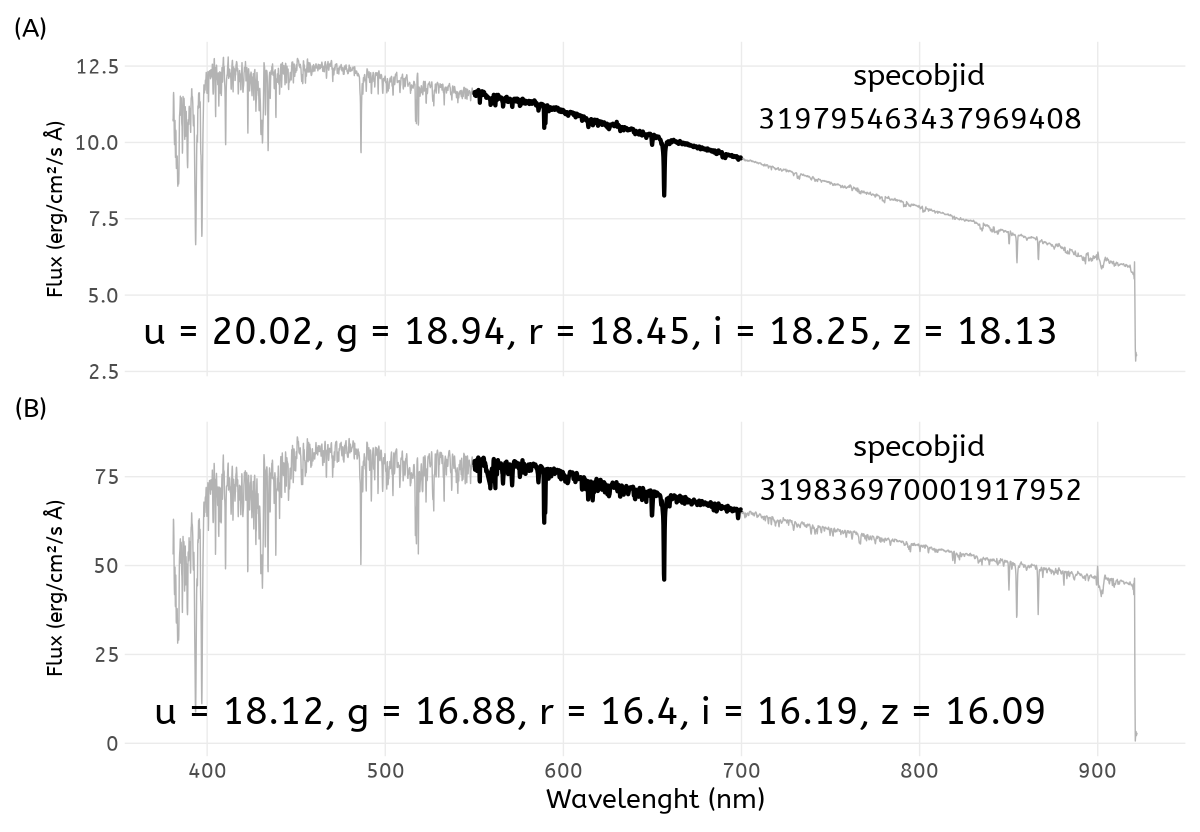
\includegraphics[width=\columnwidth, height = 8cm]{figures/spectra1}
  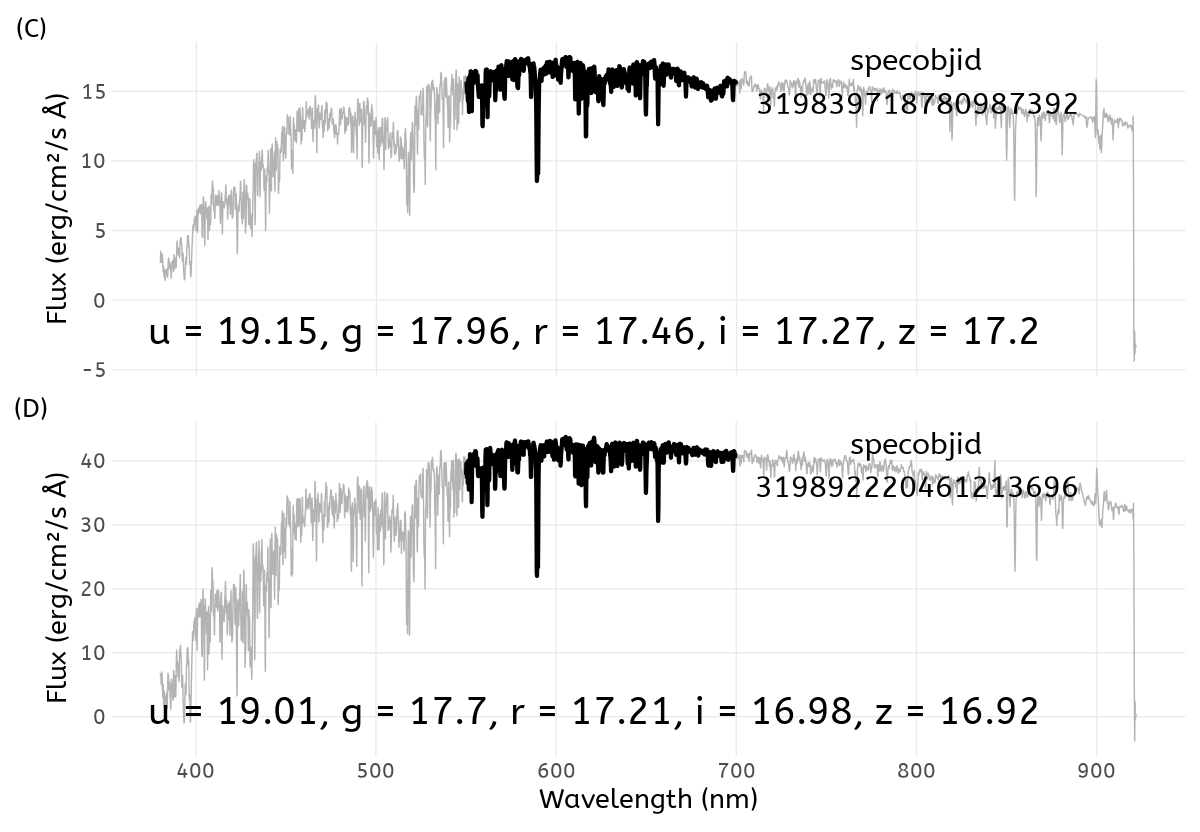
\includegraphics[width=\columnwidth, height = 8cm]{figures/spectra2}
    \caption{Two pairs of spectra downloaded from SDSS. The ugriz colour magnitudes for each star is given below its spectrum. The darkened area of the spectral line corresponds to the r-band wavelengths. The correlation between spectra A and C is 0.96. That between spectra B and D is 0.75.}
    \label{fig:spectra}
\end{figure}

Correlation is usually bounded by -1 and 1. And because these are
spectra from stars and they have similar colour magnitudes, the
correlations tend to be clustered near this higher end, see the
histogram in figure \ref{fig:histograms}A below. Machine learning
algorithms work better with normally distributed values (need reference)
and this is especially true when it comes to analysing model performance
(another reference), so the correlation values were transformed. First
of all by a logit transformation (\ref{eq:logit}):

\begin{equation}
  \displaystyle \operatorname {logit} (x)=\ln \left({\frac {1+x}{1-x}}\right)
  \label{eq:logit}
\end{equation}

And then by scaling and normalising the values to have a mean of 0 and a
standard deviation of 1. The resulting transformed values are shown in
figure \ref{fig:histograms}B.

\begin{figure}
  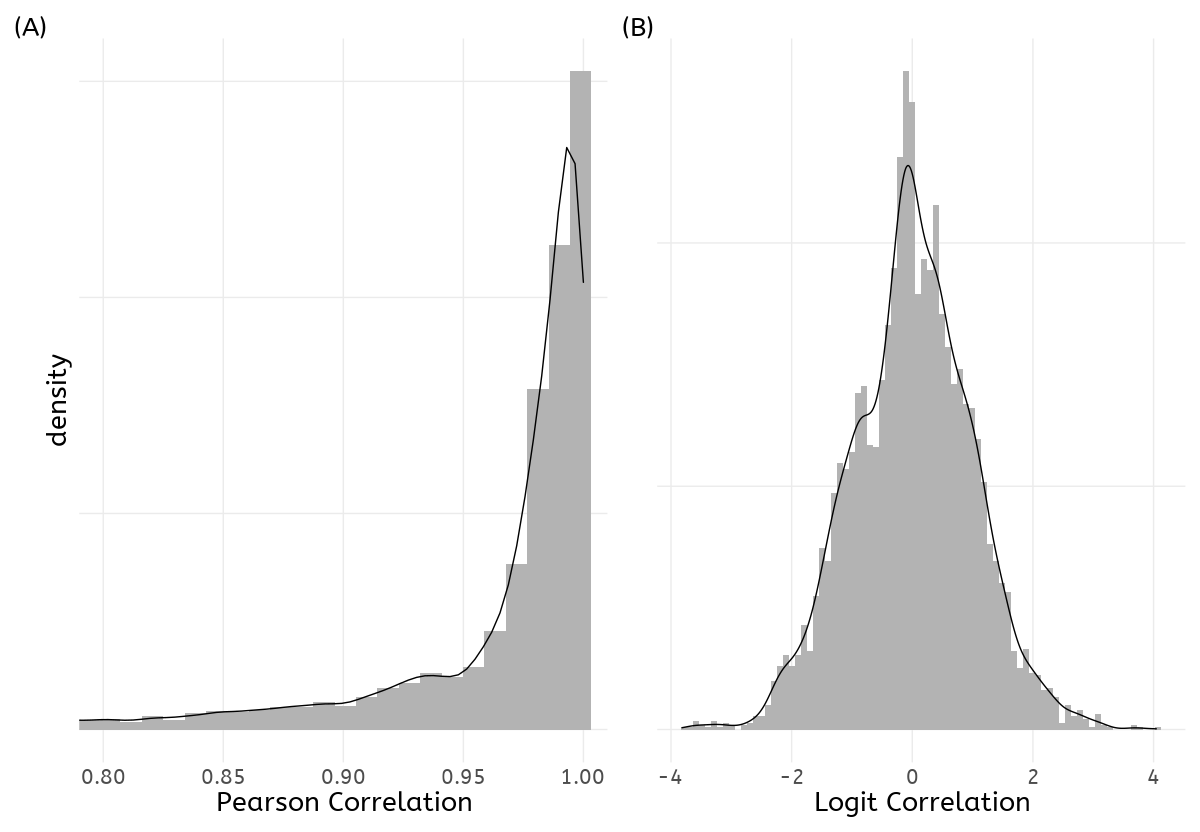
\includegraphics[width=\columnwidth, height = 5cm]{figures/histograms}
    \caption{(A) Histogram of Pearson correlation values between r-band spectra between pairs of matched stars. (B) Values in (A) transformed by a logit function.}
    \label{fig:histograms}
\end{figure}

The data is split into test and training sets, with 70\% of the data
(3915 samples) in the training set and the remainder in the test set.
Each set has a representative sample of correlation values, to do this
the original sample of 5591 pairs is split into five groups based on
percentiles of the correlation and both testing and training sets get a
commensurate proportion of each group.

\hypertarget{model}{%
\section{Model}\label{model}}

A regression model was built on the training set, using the ugriz values
for both stars in each pair as predictors for the logit(correlation)
value. An eXtreme Gradient Boosting model (Friedman, Hastie and
Tibshirani (2000), Chen and Guestrin (2021)) was used. This was chosen
because of its performance and reliability (Bentéjac, Csörgő and
Martínez-Muñoz (2020)). Cross validation was performed using a bootstrap
method (Efron (1983)). The model was fit with the maximum number of
boosting iterations set to 150, the learning rate set to 0.3, the
maximum tree depth set to 3. It was set to minimise the RMSE on the
training set. The final model fit was produced after 106 iterations.

One of the 150 trees produced is shown in figure \ref{fig:tree}.

\begin{figure}
  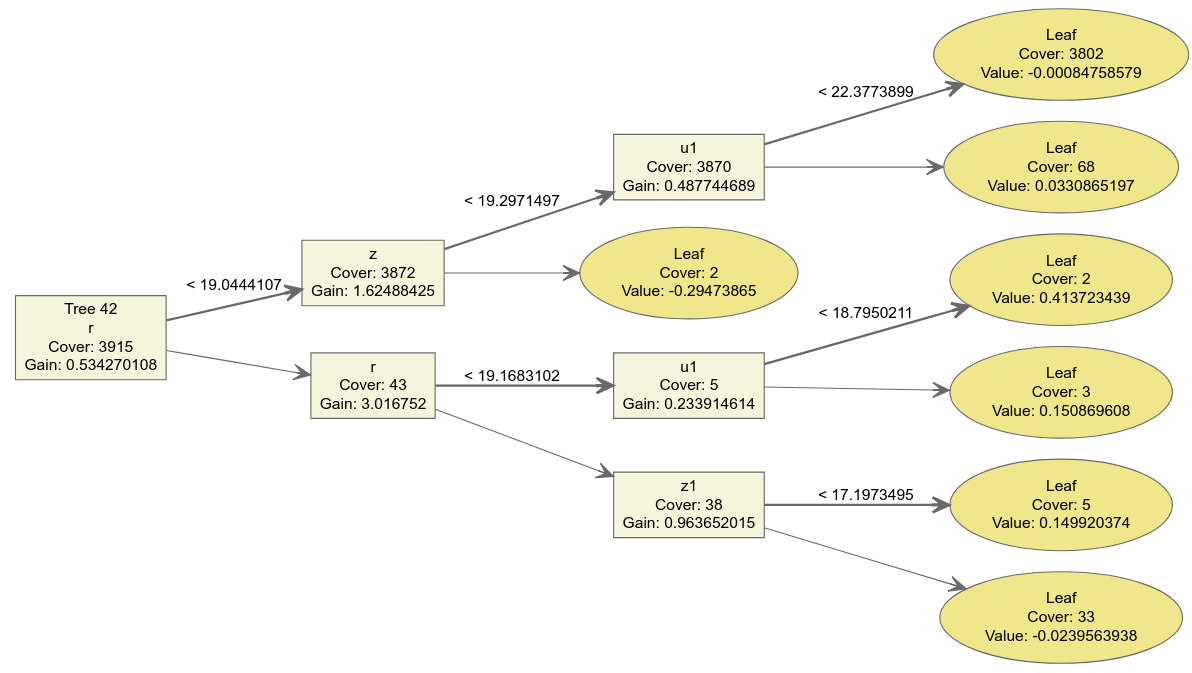
\includegraphics[width=\columnwidth, height = 6.5cm]{figures/tree}
    \caption{One of the 150 decision trees produced by the gradient boosting algorithm}
    \label{fig:tree}
\end{figure}

\hypertarget{model-evaluation}{%
\section{Model Evaluation}\label{model-evaluation}}

The model was then used to predict the logit correlation values from the
1676 star pairs from the test set. Figure \ref{fig:obs-pred} shows the
resulting values of observed logit correlation values against predicted
logit correlation values. Figure \ref{fig:residuals-pred} shows the
resulting values of the residuals, the observations minus the predicted
values, against predicted logit correlation values. Figure
\ref{fig:residuals-hist} shows a histogram of the residual values,
figure \ref{fig:residuals-qq} shows a quantile-quantile (QQ) plot of the
residuals. The shape of this last plot shows the residuals to be
somewhat platykurtic which is acceptable for a machine learning fit
(ref???).

The \(R^2\) value of predicted logit correlation on the test set was
found to be 71\%. The RMSE on the test set was found to be 0.55. The
performance of the original function used in Creaner \emph{et al.}
(2022) was worse, with an \(R^2\) of 13\%.

\begin{figure}
  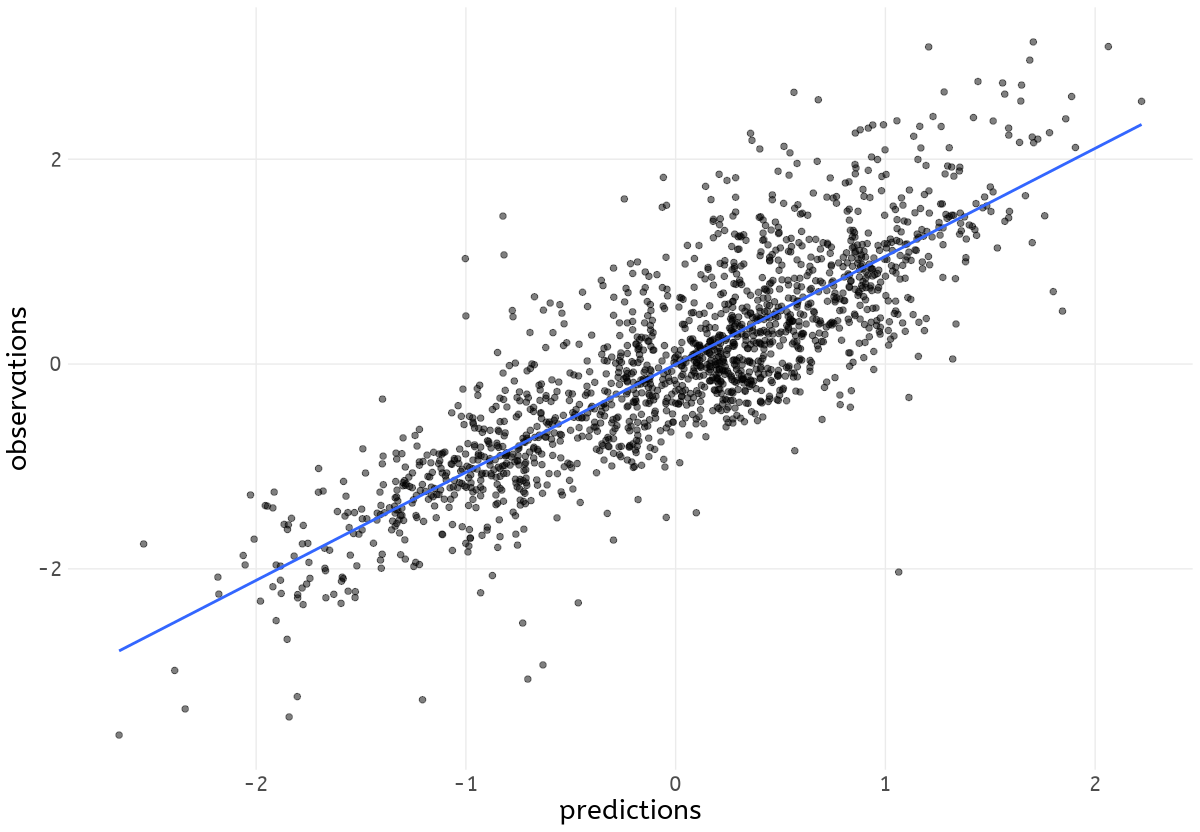
\includegraphics[width=\columnwidth, height = 6.5cm]{figures/observed-predicted}
    \caption{Observed versus predicted logit correlation values}
    \label{fig:obs-pred}
\end{figure}

\begin{figure}
  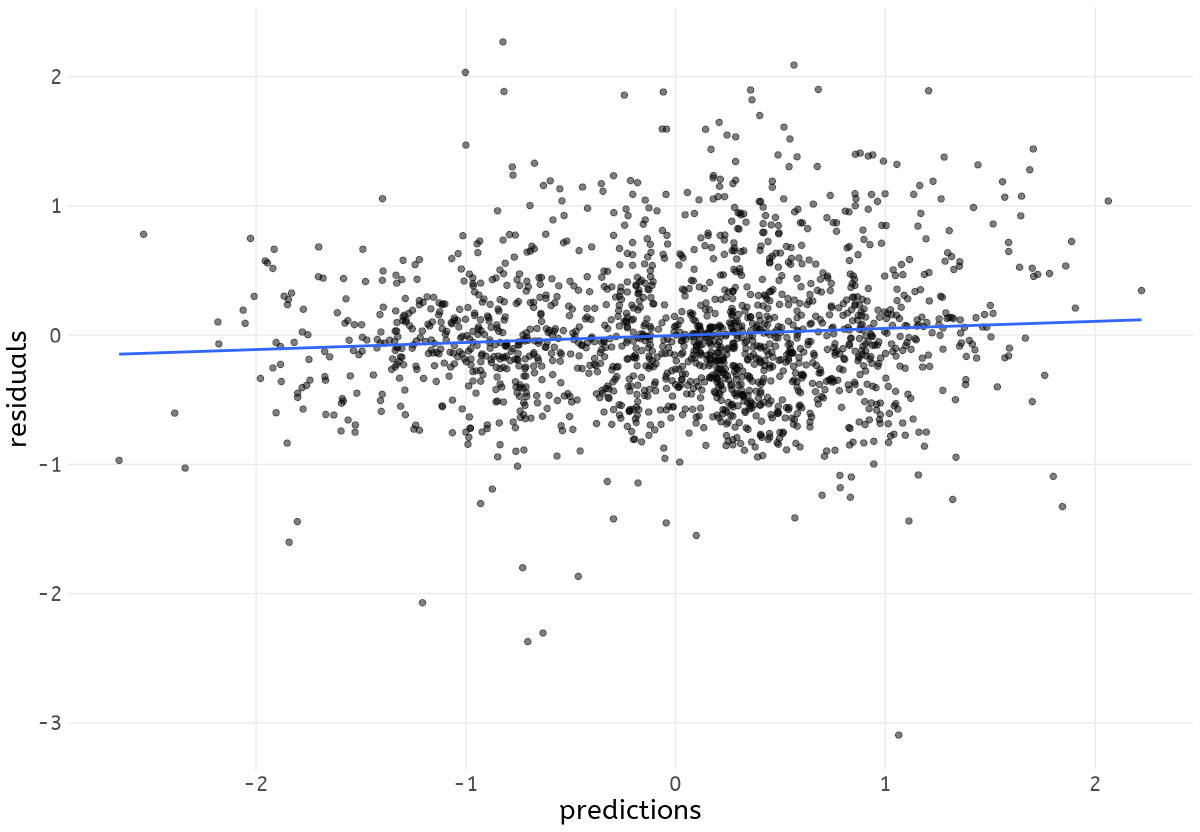
\includegraphics[width=\columnwidth, height = 6.5cm]{figures/residuals-predicted}
    \caption{Observed versus predicted logit correlation values}
    \label{fig:residuals-pred}
\end{figure}

\begin{figure}
  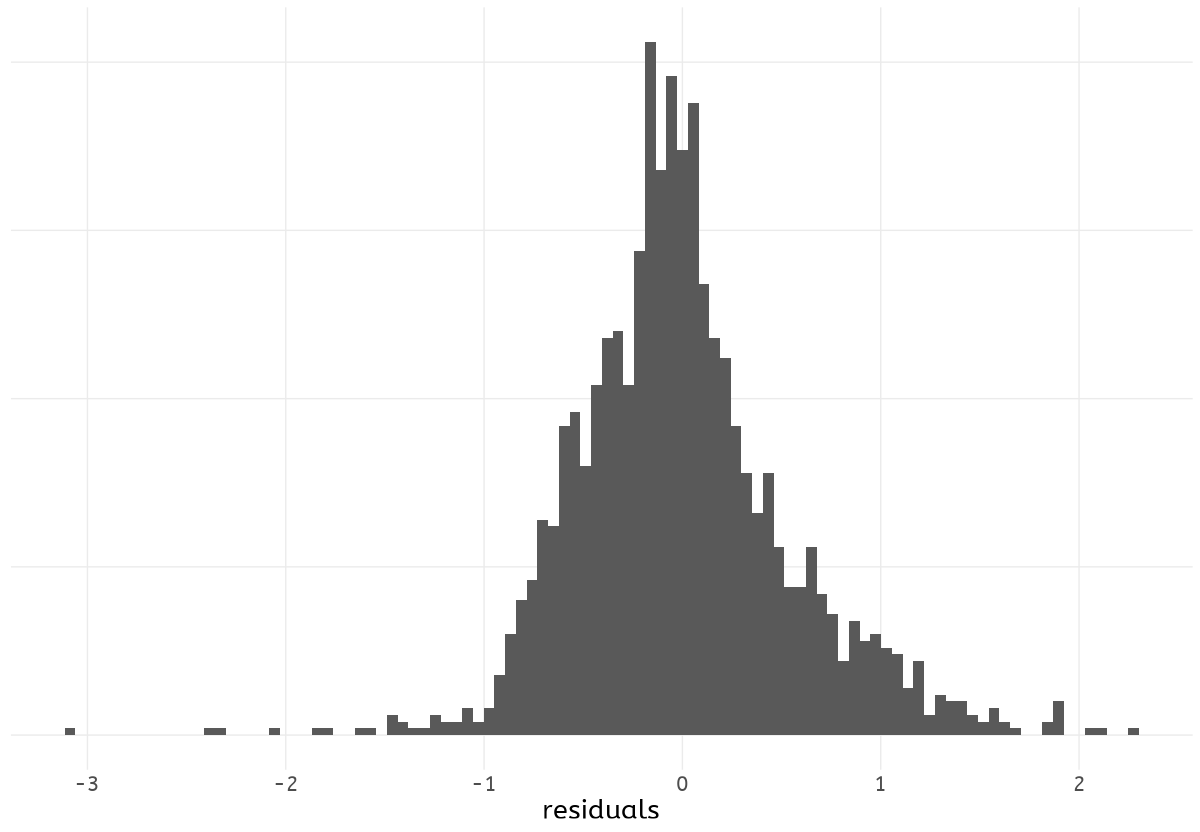
\includegraphics[width=\columnwidth, height = 6.5cm]{figures/residuals-hist}
    \caption{Observed versus predicted logit correlation values}
    \label{fig:residuals-hist}
\end{figure}

\begin{figure}
  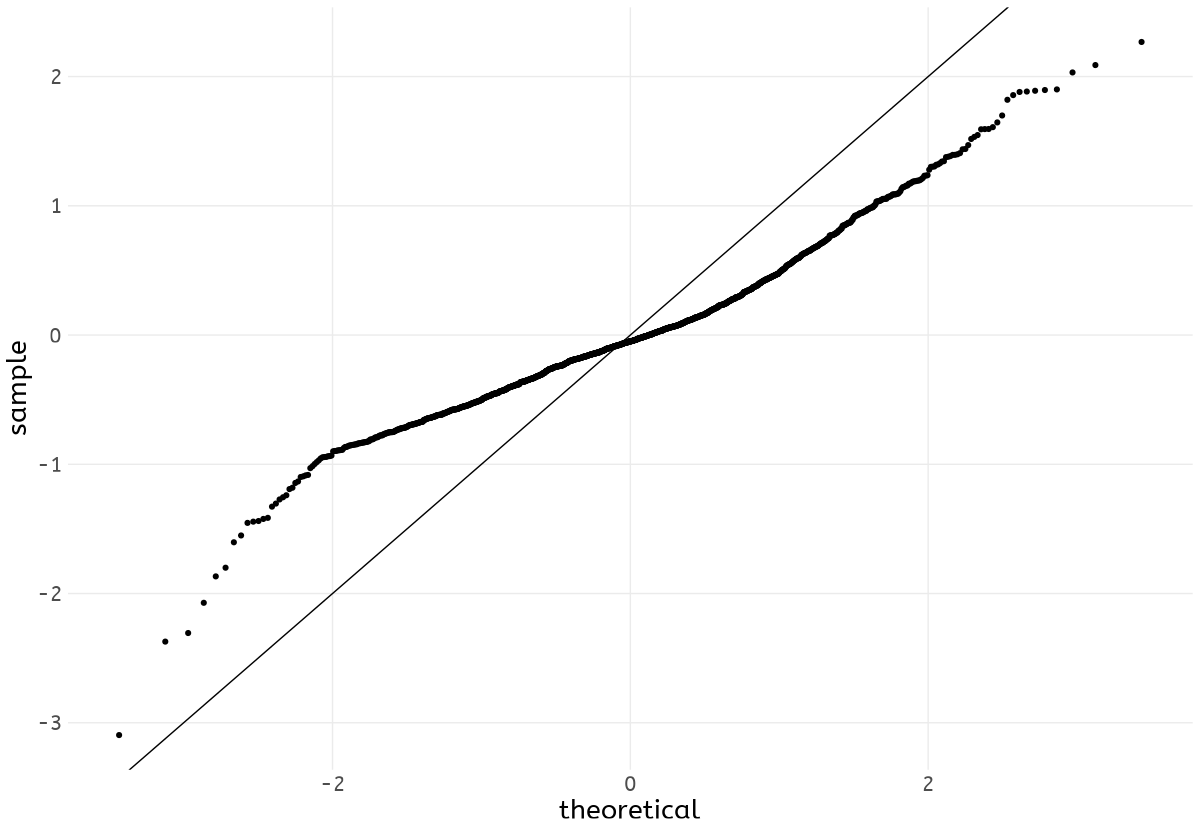
\includegraphics[width=\columnwidth, height = 6.5cm]{figures/residuals-qq}
    \caption{Observed versus predicted logit correlation values}
    \label{fig:residuals-qq}
\end{figure}

\hypertarget{conclusions}{%
\section{Conclusions}\label{conclusions}}

The last numbered section should briefly summarise what has been done,
and describe the final conclusions which the authors draw from their
work.

\hypertarget{references}{%
\section*{References}\label{references}}
\addcontentsline{toc}{section}{References}

\hypertarget{refs}{}
\begin{CSLReferences}{0}{0}
\leavevmode\vadjust pre{\hypertarget{ref-Aguado2018}{}}%
Aguado, D.S. \emph{et al.} (2018) {``{The Fifteenth Data Release of the
Sloan Digital Sky Surveys: First Release of MaNGA Derived Quantities,
Data Visualization Tools and Stellar Library}.''}
doi:\href{https://doi.org/10.3847/1538-4365/aaf651}{10.3847/1538-4365/aaf651}.

\leavevmode\vadjust pre{\hypertarget{ref-Bentejac2020}{}}%
Bentéjac, C., Csörgő, A. and Martínez-Muñoz, G. (2020) {``{A comparative
analysis of gradient boosting algorithms},''} \emph{Artificial
Intelligence Review 2020 54:3}, 54(3), pp. 1937--1967.
doi:\href{https://doi.org/10.1007/S10462-020-09896-5}{10.1007/S10462-020-09896-5}.

\leavevmode\vadjust pre{\hypertarget{ref-Burdanov2014}{}}%
Burdanov, A.Y., Krushinsky, V.V. and Popov, A.A. (2014) {``{Astrokit-an
Efficient Program for High-Precision Differential CCD Photometry and
Search for Variable Stars},''} \emph{Translated from Astrofizicheskij
Byulleten}, 69(3). Available at:
\url{https://arxiv.org/abs/1408.0664v1}.

\leavevmode\vadjust pre{\hypertarget{ref-Chen2021}{}}%
Chen, T. and Guestrin, C. (2021) {``{Extreme Gradient Boosting {[}R
package xgboost version 1.5.0.2{]}},''} \emph{Proceedings of the ACM
SIGKDD International Conference on Knowledge Discovery and Data Mining},
13-17-Augu, pp. 785--794.
doi:\href{https://doi.org/10.1145/2939672.2939785}{10.1145/2939672.2939785}.

\leavevmode\vadjust pre{\hypertarget{ref-creaner2020}{}}%
Creaner, O. \emph{et al.} (2020) {``{A catalogue of Locus Algorithm
pointings for optimal differential photometry for 23 779 quasars},''}
\emph{Monthly Notices of the Royal Astronomical Society}, 498(3), pp.
3720--3729.
doi:\href{https://doi.org/10.1093/MNRAS/STAA2494}{10.1093/MNRAS/STAA2494}.

\leavevmode\vadjust pre{\hypertarget{ref-creaner2022}{}}%
Creaner, O. \emph{et al.} (2022) {``{The Locus Algorithm: A novel
technique for identifying optimised pointings for differential
photometry},''} \emph{Astronomy and Computing}, 38, p. 100537.
doi:\href{https://doi.org/10.1016/J.ASCOM.2021.100537}{10.1016/J.ASCOM.2021.100537}.

\leavevmode\vadjust pre{\hypertarget{ref-Creaner2017}{}}%
Creaner {[}Thesis{]}, O. (2017) {``{Data Mining by Grid Computing in the
Search for Extrasolar Planets},''} \emph{Doctoral} {[}Preprint{]}.
doi:\url{https://doi.org/10.21427/7w45-6018}.

\leavevmode\vadjust pre{\hypertarget{ref-Efron1983}{}}%
Efron, B. (1983) {``{Estimating the error rate of a prediction rule:
Improvement on cross-validation},''} \emph{Journal of the American
Statistical Association}, 78(382), pp. 316--331.
doi:\href{https://doi.org/10.1080/01621459.1983.10477973}{10.1080/01621459.1983.10477973}.

\leavevmode\vadjust pre{\hypertarget{ref-Everett2001}{}}%
Everett, M.E. and Howell, S.B. (2001) {``{A Technique for
Ultrahigh‐Precision CCD Photometry},''} \emph{Publications of the
Astronomical Society of the Pacific}, 113(789), pp. 1428--1435.
doi:\href{https://doi.org/10.1086/323387/0}{10.1086/323387/0}.

\leavevmode\vadjust pre{\hypertarget{ref-Friedman2000}{}}%
Friedman, J., Hastie, T. and Tibshirani, R. (2000) {``{Additive logistic
regression: A statistical view of boosting},''} \emph{Annals of
Statistics}, 28(2), pp. 337--407.
doi:\href{https://doi.org/10.1214/AOS/1016218223}{10.1214/AOS/1016218223}.

\leavevmode\vadjust pre{\hypertarget{ref-Giltinan2011}{}}%
Giltinan, A. \emph{et al.} (2011) {``{Using EMCCD's to improve the
photometric precision of ground-based astronomical observations},''}
\emph{Journal of Physics: Conference Series}, 307(1).
doi:\href{https://doi.org/10.1088/1742-6596/307/1/012010}{10.1088/1742-6596/307/1/012010}.

\leavevmode\vadjust pre{\hypertarget{ref-Milone2011a}{}}%
Milone, E.F. and Pel, J.W. (2011) {``{The High Road to Astronomical
Photometric Precision: Differential Photometry},''} pp. 33--68.
doi:\href{https://doi.org/10.1007/978-1-4419-8050-2_2}{10.1007/978-1-4419-8050-2\_2}.

\leavevmode\vadjust pre{\hypertarget{ref-Smith2008}{}}%
Smith, N. \emph{et al.} (2008) {``{EMCCD Technology in High Precision
Photometry on Short Timescales},''} \emph{ASSL}, 351, p. 257.
doi:\href{https://doi.org/10.1007/978-1-4020-6518-7_13}{10.1007/978-1-4020-6518-7\_13}.

\leavevmode\vadjust pre{\hypertarget{ref-Sterken2011}{}}%
Sterken, C., Milone, E.F. and Young, A.T. (2011) {``{Photometric
Precision and Accuracy},''} pp. 1--32.
doi:\href{https://doi.org/10.1007/978-1-4419-8050-2_1}{10.1007/978-1-4419-8050-2\_1}.

\end{CSLReferences}

\appendix

\hypertarget{some-extra-material}{%
\section{Some extra material}\label{some-extra-material}}

If you want to present additional material which would interrupt the
flow of the main paper, it can be placed in an Appendix which appears
after the list of references.

%%%%%%%%%%%%%%%%%%%%%%%%%%%%%%%%%%%%%%%%%%%%%%%%%%


% Don't change these lines
\bsp	% typesetting comment
\label{lastpage}
\end{document}


% End of mnras_template.tex
